\documentclass[11pt, oneside]{book}

% URLs and hyperlinks ---------------------------------------
\usepackage{hyperref}
\hypersetup{
	colorlinks=true,
	linkcolor=blue,
	filecolor=magenta,      
	urlcolor=blue,
}
\usepackage{xurl}
%---------------------------------------------------

% titlepage -------------------------------------------------
\usepackage{pdfpages}
%------------------------------------------------------------

% tables -------------------------------------------------------
\usepackage{float}
\usepackage{multirow}
\renewcommand{\arraystretch}{1.23}
% ---------------------------------------------------------------------

% commands --------------------------------------------
\newcommand{\amz}{\lr{Amazon} }
% -----------------------------------------------------------

\usepackage{xepersian}
\settextfont{Yas}
\setdigitfont{Yas}

\begin{document}
\frontmatter
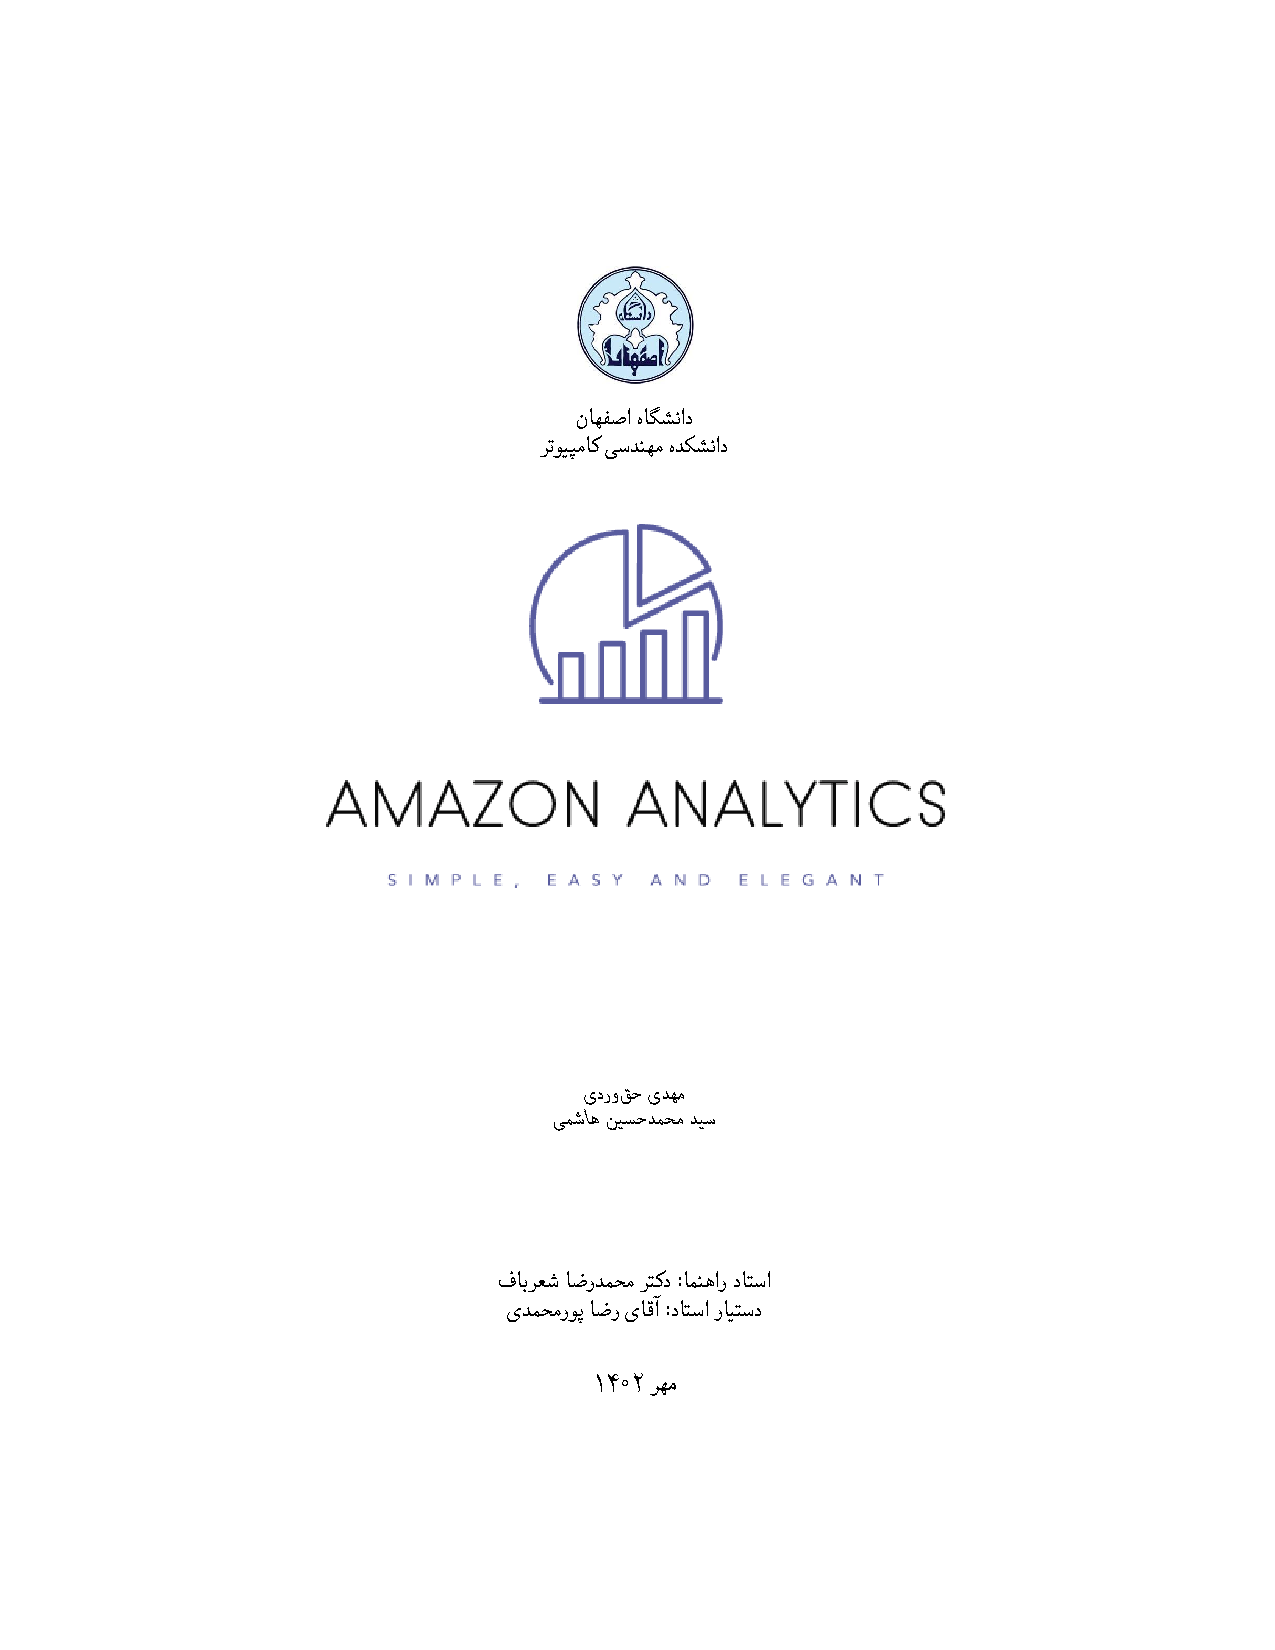
\includepdf{../titlepage/title}
\tableofcontents
\mainmatter

\chapter{معرفی}
    پس از بررسی مواردی که برای پیاده‌سازی ارائه شده بود، موضوع \textit{منابع انسانی:‌ سیستم ارزیابی عملکرد کارمندان} انتخاب گردید.
    
    به طور خلاصه این سیستم قرار است طبق چارت سازمانی معرفی شده در ادامه‌ی این سند، خدمات آماری به همراه جزئیات، به شرکت \amz و مدیران آن ارائه دهد. 
    
    داده‌های مورد نیاز این خدمات آماری از آمار‌های ارائه شده توسط خود شرکت \amz و تمامی بازخورد (\lr{feedback})های مشتریان آن، جمع‌آوری و استفاده می‌شوند.
    
    بر این اساس چون این سیستم قرار است به بررسی عملکرد کارمندان شرکت \amz بپردازد، و خدماتی که ارائه می‌دهد، خدمات آماری هستند، نام \lr{\textit{Amazon Analytics}} برای آن انتخاب گردید.
\chapter{مدل تجاری \lr{(Business Case)}}
\section{جدول \lr{RACI}}
\begin{table}[H]
    \begin{latin}
        \begin{center}
            \begin{tabular}{|c|c|c|}
                \hline
                Task/Person & Mahdi & Seyed Mohammad Hussein \\
                \hline
                \hline
                Project Goals & R/A/C/I & R/A/C/I \\
                \hline
                ... & ... & ... \\
                \hline
            \end{tabular}
        \end{center}
    \end{latin}
\end{table}

\section{ماتریس تصمیم‌گیری راهبری}
\begin{table}[H]\caption{\lr{Does the strategy meet the required objectives?}}
    \begin{latin}
        \begin{center}
            \begin{tabular}{|c|c|c|c|c|}
                    \hline
                    \multirow{2}{*}{Required Objectives}
                     & \multicolumn{4}{|c|}{Strategies} \\
                     \cline{2-5}
                    & 1 & 2 & 3 & 4 \\
                    \hline
                    Fuckin the new CEO & No & Yes & No & Yes \\
                    \hline
                    Marry the secretary & Yes & Yes & No & No \\
                    \hline
            \end{tabular}
        \end{center}
    \end{latin}
\end{table}

\begin{table}[H]\caption{\lr{How likely is this strategy to meet the other objectives?}}
    \begin{latin}
        \begin{center}
            \begin{tabular}{|c|c|c|c|c|c|}
                \hline
                \multirow{2}{*}{Other objectives} &
                \multirow{2}{*}{Importance} &
                \multicolumn{4}{|c|}{Strategies}\\
                \cline{3-6}
                & & 2 & 3 & 4 & 5 \\
                \hline
                Welcome to the fukcing new commers &
                5 & 
                &
                &
                1
                &
                5 \\
                \hline
                \textbf{Total} & & 0& 0 & 2 & 5 \\
                \hline
            \end{tabular}
        \end{center}
    \end{latin}
\end{table}
\chapter{پیاده‌سازی نسخه‌ی دمو}
\chapter{قالب \lr{Brainstorming}}
\end{document}